\section{Исследовательский раздел}

На рисунке \ref{fig:insmod} показан лог загрузки модуля.

\begin{figure}[h!btp]
	\centering
	\includegraphics[width=0.9\textwidth]{inc/insmod.png}
	\caption{Загрузка модуля}
	\label{fig:insmod}
\end{figure}

На рисунке \ref{fig:init} показан лог инициализации команд.

\begin{figure}[h!btp]
	\centering
	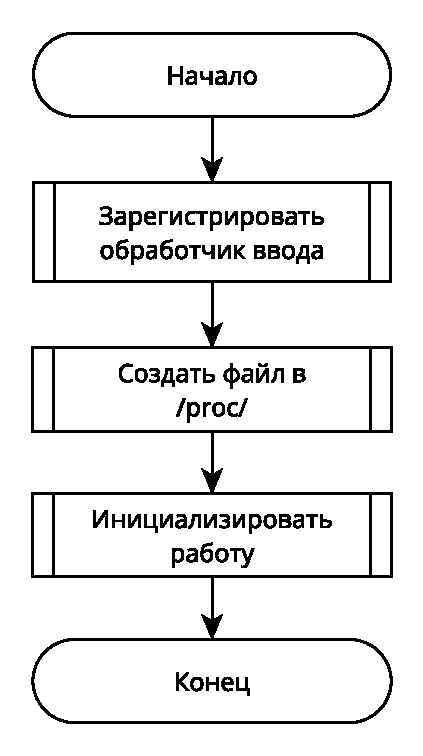
\includegraphics[width=0.9\textwidth]{inc/init.png}
	\caption{Инициализация команд}
	\label{fig:init}
\end{figure}

На рисунке \ref{fig:proc_file} показана проверка файла в /proc/.

\begin{figure}[h!btp]
	\centering
	\includegraphics[width=0.7\textwidth]{inc/proc\_file.png}
	\caption{Проверка файла в /proc/}
	\label{fig:proc_file}
\end{figure}

На рисунке \ref{fig:work_example} показан пример успешной работы.

\begin{figure}[H]
	\centering
	\includegraphics[width=0.8\textwidth]{inc/work\_example.png}
	\caption{Пример работы}
	\label{fig:work_example}
\end{figure}

На рисунке \ref{fig:unknown_gesture} показана обработка неизвестного шаблона движения.

\begin{figure}[H]
	\centering
	\includegraphics[width=0.8\textwidth]{inc/unknown_gesture.png}
	\caption{Неизвестный шаблон}
	\label{fig:unknown_gesture}
\end{figure}

На рисунке \ref{fig:rmmod} показана выгрузка модуля.

\begin{figure}[H]
	\centering
	\includegraphics[width=0.8\textwidth]{inc/rmmod.png}
	\caption{Выгрузка модуля}
	\label{fig:rmmod}
\end{figure}

\clearpage